\documentclass[12pt]{article}
\usepackage[a4paper,margin=1in]{geometry}
\usepackage[utf8]{inputenc}
\usepackage[T1]{fontenc}
\usepackage{setspace}
\usepackage{natbib}
\usepackage{booktabs}
\usepackage{graphicx}
\usepackage{amsmath}
\usepackage{amssymb}
\usepackage{hyperref}
\usepackage{caption}
\usepackage{threeparttable}
\hypersetup{colorlinks=true, linkcolor=blue, citecolor=blue, urlcolor=blue}
\setstretch{1.5}
\bibliographystyle{apalike}
\setlength{\textfloatsep}{8pt plus 2pt minus 2pt}
\setlength{\floatsep}{6pt plus 2pt minus 2pt}
\setlength{\intextsep}{6pt plus 2pt minus 2pt}
\setlength{\abovecaptionskip}{4pt}
\setlength{\belowcaptionskip}{2pt}
\raggedbottom

\title{\textbf{The Quantity and Size of Microloans Follow Different Development Logics:\\
Evidence from Kiva}}
\author{Kexing Yan \\ \textit{University of Toronto}}
\date{\today}

\begin{document}
\maketitle

\begin{abstract}
\noindent
I study how Kiva microfinance activity relates to economic development across an 84-country panel
(2013--2017), testing whether lending follows the inverted-U (``middle-income peak'') pattern
suggested by early descriptive plots, and at which of three margins. Conditional on Kiva already
lending in a country, total volume shows no significant nonlinearity (quadratic $p=0.179$), confirmed
by a formal Lind--Mehlum (2010) shape test. At the loan level, individual loan size follows a
significant \emph{U-shape} ($p<0.001$), the opposite sign, which the same formal test confirms
decisively. At the \emph{extensive} margin --- whether Kiva operates in a country at all, on a global
panel including zero-lending country-years --- a Logit model finds significant concavity (quadratic
$p=0.023$), but the same shape test shows the initial rise in entry probability among the poorest
countries is not statistically distinguishable from flat, so a completed inverted-U is not formally
established. The contribution is documenting this three-way divergence while holding every margin,
including the paper's most favorable-looking result, to one formal shape-test standard rather than
reading significance off a single quadratic coefficient.

\vspace{0.5cm}
\noindent \textbf{JEL Codes:} G21, O16, O12

\noindent \textbf{Keywords:} microfinance; Kiva; economic development; extensive margin; PPML;
U-test
\end{abstract}

\doublespacing
\setstretch{1.5}

\section{Introduction}

Microfinance is often described as a tool for expanding credit access where formal banking systems
are thin, but the empirical literature does not support a simple view that more poverty automatically
implies more successful microfinance. Early survey and review work emphasizes both the promise and
the limits of microfinance, especially the tension between outreach to poor borrowers and the
operational realities of lending in weak institutional environments \citep{morduch1999}. A second
strand of work studies microfinance institutions directly and argues that financial sustainability,
commercialization, and outreach often move together only imperfectly. \citet{cull2007} and
\citet{cull2009} show that institutions can scale, but doing so may involve trade-offs between
profitability and reaching poorer clients. \citet{hermes2011} similarly find that deeper outreach can
be associated with lower operating efficiency.

A third strand asks whether microcredit actually improves welfare for poor households. Some
influential studies report gains in access to credit and business activity but more limited average
effects on broader welfare outcomes. \citet{banerjee2015}, \citet{angelucci2015},
\citet{tarozzi2015}, and \citet{karlanzinman2011} all contribute to a more cautious consensus:
microcredit may help some borrowers and relax constraints, but average poverty effects are not
universally large or immediate. This more skeptical perspective is reinforced by replication and
reanalysis work such as \citet{roodman2014}, which highlights how sensitive headline claims can be to
identification choices and model specification. At the same time, classic work on financial access
and poverty, such as \citet{pitt1998} and \citet{burgess2005}, keeps attention on the idea that
credit access can matter, especially when it expands into underserved places. Platform-mediated
peer-to-peer giving of the kind Kiva popularized adds a further wrinkle: lender-side motivations and
platform design shape which borrowers and loan types get funded in ways that are distinct from
traditional microfinance institutions \citep{galak2011}.

Taken together, this literature offers three recurring lessons that motivate the empirical strategy
below. First, outreach to poor borrowers and financial sustainability are not automatically aligned, so
where and how intensively a lender operates cannot be read off a single summary statistic. Second, the
average treatment effects documented at the household level do not by themselves say anything about
the geographic allocation of lending activity across countries at different stages of development ---
a platform can expand into a country for reasons that have little to do with the marginal welfare gain
to any individual borrower there. Third, the RCT literature's emphasis on careful identification of a
single causal object stands in useful contrast to a question this paper treats as explicitly
non-causal and multi-object: not ``does microcredit help,'' but ``at which of several distinct margins
does microfinance activity vary with development, and in which direction.''

These papers are highly relevant, but most focus on either household-level treatment effects or
institution-level performance. This paper asks a different question at the country-year and loan
level: where is platform-based microfinance most active across countries, and does the answer depend
on whether ``activity'' is measured by whether Kiva operates there at all, by total volume, or by the
size of individual loans? Country-level Kiva lending data capture the geographic allocation of
microfinance activity rather than only average borrower outcomes or the internal efficiency of a
single lender; a global panel that adds zero-lending country-years lets the same question be asked
about the \emph{extensive} margin (does Kiva operate in a country at all); and loan-level data let it
be asked about the \emph{intensive} margin --- how large a loan Kiva borrowers receive, conditional on
receiving one.

The analysis uses an $X \to Y \to Z$ framework, with three versions of $Y$. The first, \emph{Kiva
presence}, captures whether Kiva lends in a country-year at all. The second, \emph{total lending
volume}, captures how much Kiva activity a country receives conditional on Kiva being present. The
third, \emph{individual loan size}, captures how large a typical loan is once a loan has been made.
The main explanatory variable $X$ is economic development, proxied by log GDP per capita. The
mechanism $Z$ is institutional quality and financial access, which may shape whether development
translates into more or less microfinance activity. Kiva lending data are combined with World Bank
macroeconomic indicators, governance variables, and country-level population measures to build all
three panels.

Initial descriptive plots (Section~\ref{sec:descriptive}) suggest a possible middle-income hump in
total lending volume, which motivated an original hypothesis that lending follows an inverted-U
pattern peaking in lower-middle income countries. That hypothesis does not survive formal regression
testing at the country level (Section~\ref{sec:results-country}) conditional on Kiva already operating
there: the quadratic term is never significant, a conclusion confirmed by a formal shape test
(Section~\ref{sec:utest}). What the data \emph{do} support, robustly, is a divergence across margins:
whether Kiva enters a country at all is significantly concave in development, with entry probability
falling steeply with income, though the initial rise among the very poorest does not pass the formal
low-end slope test; total lending volume conditional on entry trends flat-to-downward with
development; and the size of individual loans follows a significant U-shape --- falling and then
rising with income. The remainder of the paper develops these three results, checks their robustness,
and discusses limitations, including that the size and quantity margins remain descriptive, non-causal
analyses of countries and loans that Kiva has already chosen to serve.

\section{Data}
\label{sec:data}

\subsection{Construction}

The central empirical question is whether Kiva lending activity is concentrated in the poorest
countries, clusters at intermediate development levels, or instead varies with development in some
other way --- and whether that answer changes depending on whether ``activity'' means total volume or
typical loan size. The main dataset begins with Kiva loan-level posting records
\citep{kiva_data} and aggregates them to the \textbf{country-year} level for 2013--2017: loan amounts
and loan counts are summed within each country-year and merged with country-level development and
institutional variables. A second, loan-level file keeps each individual loan as its own observation
and merges in the same country-year covariates.

The country-year panel's main variables are: \textbf{quantity} (total Kiva lending activity, log
total loan amount); \textbf{size} (individual loan size, loan level only, log loan amount);
\textbf{development} ($X$, log GDP per capita); \textbf{institutional environment} ($Z$, an
institutional-quality principal component, with an alternative index and a financial-access index as
robustness measures); and \textbf{controls}, especially log population, to account for country size.
Poverty rate is used only in a limited-sample descriptive check, given substantial missingness; a
broader cleaned dataset also carries measures such as the Human Development Index, life expectancy, and
gross national income where available, though these are not part of the main regression battery. Before
estimation, the merged panel is audited for duplicate country-year keys, variable missingness, and
within-country variation, since the analysis depends on correct country-code/year merges and some
merged variables are available for fewer observations than the Kiva outcome itself; this audit step
matters in practice, since it is what first flags that the institutional-quality series are the most
missingness-prone inputs into the regressions below, well before any model is estimated.

\subsection{External Data and Merging}

These outside datasets are essential because the Kiva records describe lending activity but do not by
themselves measure cross-country development, institutional quality, or population size. The Kiva
panel is enriched with three external sources from the World Bank's World Development Indicators
\citep{worldbank_wdi}, merged at the country-year level by country code and year. First, GDP-per-capita
data (constant 2015 USD) construct the main development regressor. Second, governance and
financial-development indicators construct the institutional-quality principal component and its two
alternative measures; these capture dimensions of institutional strength, governance quality, and
access to formal financial infrastructure, and play the role of the mechanism variable $Z$. Because
these series are incomplete or nearly time-invariant over 2013--2017 for some countries, all three
measures are reported and compared rather than relying on a single one. Third, country-level
demographic and development controls, especially population, are merged in; population is particularly
important because raw loan totals partly reflect country size, so per-capita measures are needed to
avoid conflating scale with lending intensity. The panel audit described above reports duplicate
country-year keys, missingness after merging, and within-country variation in the merged variables,
which is why the three institutional measures are compared side by side rather than treated as
interchangeable.

\subsection{Sample Period: Is 2013 Comparable?}
\label{sec:sample-period}

The panel begins in 2013, when Kiva's own posting volume was still ramping up, so before treating the
2013--2017 year fixed effects in Section~\ref{sec:results} as evidence of anything, it is worth
checking directly whether 2013 is a genuinely comparable observation year. A decision rule, applied
mechanically before looking at any regression results, treats 2013 as \emph{incomplete} and drops it
if either (a) fewer than 10 of 12 months are represented in the raw loan-posting dates, or (b) loan
counts are below 40\% of 2014's \emph{and} country coverage is clearly lower than 2014's. Table
\ref{tab:tableA1} in the Appendix, built directly from raw loan-posting timestamps rather than the
aggregated panel, shows 2013 has complete 12-month coverage, loan counts 80.4\% of 2014's (above the
40\% threshold), and country coverage of 74 versus 81 in 2014 (not ``clearly lower''). Neither
disqualifying condition is met, so the full 2013--2017 sample is retained, with lower 2013 activity
levels read as genuine platform growth rather than a partial-year artifact. This motivates including
year fixed effects in the preferred specifications rather than treating them as a nuisance control;
Section~\ref{sec:robustness} re-estimates the preferred specifications on the 2014--2017 subsample
only as a direct check on this judgment call.

\section{Descriptive Evidence}
\label{sec:descriptive}

Table \ref{tab:table1} reports summary statistics for the core regression variables. The sample spans
substantial variation in both development and lending intensity: log GDP per capita covers low-income
through relatively rich economies, log total loan amount shows Kiva lending is far from uniform across
countries, and the institutional and financial-access variables display meaningful cross-country
dispersion. A first, purely descriptive cut splits total lending by development tercile (Table
\ref{tab:table2}, Appendix): the middle-development tercile has the highest mean log lending (13.436)
compared to the low- (12.806) and high-development terciles (12.776). This raw, bivariate pattern is
the origin of the original middle-income-peak hypothesis and motivates taking it seriously as a
starting point, but as Section~\ref{sec:results-country} shows, it does not survive as a statistically
significant nonlinear relationship once the regressions control for institutions, population, and year
effects and formally test the quadratic term.

Figure \ref{fig:fig1} plots the main bivariate relationship between development and total lending
volume, with a quadratic fit and a LOWESS smoother overlaid on the raw country-year scatter. Both
curves bend downward at higher income levels, which is the descriptive origin of the middle-income-peak
hypothesis and is worth taking seriously as a starting point. This is, however, still purely
unconditional evidence: it does not control for institutions, population, or year, and
Section~\ref{sec:results-country} shows the same curvature is not statistically significant once those
controls and a formal shape test are added. Figure \ref{fig:fig2} shows the distribution of the
dependent variable itself, which is far from tightly clustered --- substantial heterogeneity in lending
across country-years is what gives the later regressions meaningful cross-country variation to work
with, rather than only a handful of outlying observations driving the result. Figure \ref{fig:fig3}
shows the distribution of log GDP per capita across the sample, confirming that the panel covers a wide
development range, from low-income to relatively rich economies; that breadth is necessary for asking
whether the development--microfinance relationship is monotonic, nonlinear, or different across the
quantity and size margins in the first place.

Figure \ref{fig:fig4} rescales lending by population, using loan amount per 100,000 people rather than
raw country totals, which reduces the risk of mechanically reading large countries as high-lending
simply because they are large; the per-capita pattern is broadly similar in shape to Figure
\ref{fig:fig1}. Figures \ref{fig:fig5}--\ref{fig:fig7} then map average lending, development, and
institutional quality across countries over 2013--2017. The goal of the maps is not causal
identification but a check that the geography of microfinance is visually consistent with the
bivariate patterns above: Figure \ref{fig:fig5} maps the per-capita outcome, Figure \ref{fig:fig6} maps
the main development regressor, and Figure \ref{fig:fig7} maps the institutional mechanism. All three
are built using the underlying shapefile's alternate ISO code field rather than its primary one,
because the primary field codes several territories with complex sovereignty status (including
Kosovo, which is Kiva-active in this panel) as a single non-standard placeholder value; using the
alternate field restores those countries' outlines to the map rather than leaving unexplained holes in
the choropleth, so that grey areas on the map can be read as genuine ``no Kiva data'' rather than a
plotting artifact.

\begin{table}[htbp]
\centering
\caption{Summary Statistics (Country-Year Panel)}
\label{tab:table1}
\resizebox{\textwidth}{!}{%
\begin{tabular}{lcccccc}
\toprule
Variable & N & Mean & SD & Min & Median & Max \\
\midrule
Log Total Loan Amount & 357.000 & 12.955 & 1.933 & 7.151 & 13.137 & 16.602 \\
Log GDP per capita & 351.000 & 7.834 & 1.067 & 5.539 & 7.776 & 10.971 \\
Institutional quality (PCA1) & 352.000 & -0.132 & 0.884 & -2.551 & -0.085 & 1.955 \\
Institutional quality index & 352.000 & -0.115 & 0.803 & -2.325 & -0.075 & 1.898 \\
Financial access index & 323.000 & 0.069 & 1.095 & -0.945 & -0.145 & 6.861 \\
Log population & 354.000 & 16.640 & 1.617 & 12.188 & 16.588 & 21.067 \\
Poverty Rate & 151.000 & 11.797 & 17.016 & 0.000 & 4.800 & 75.800 \\
\bottomrule
\end{tabular}%
}
\par\smallskip\footnotesize Country-year panel, $N=357$ observations across 84 countries, 2013--2017.
\end{table}

\begin{figure}[htbp]
\centering
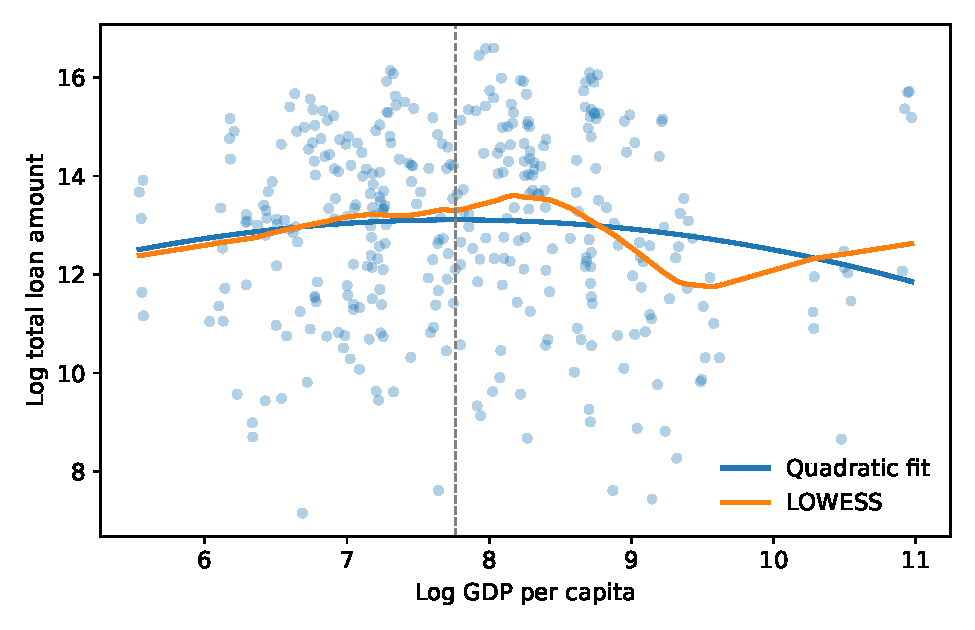
\includegraphics[width=0.75\textwidth]{figures/figure1_scatter_quadratic.pdf}
\caption{Development and total lending volume. Each point is one country-year; the solid curve is a
quadratic fit and the dashed curve a LOWESS smoother, both fit without controls. The vertical dashed
line marks the quadratic fit's implied turning point.}
\label{fig:fig1}
\end{figure}

\begin{figure}[htbp]
\centering
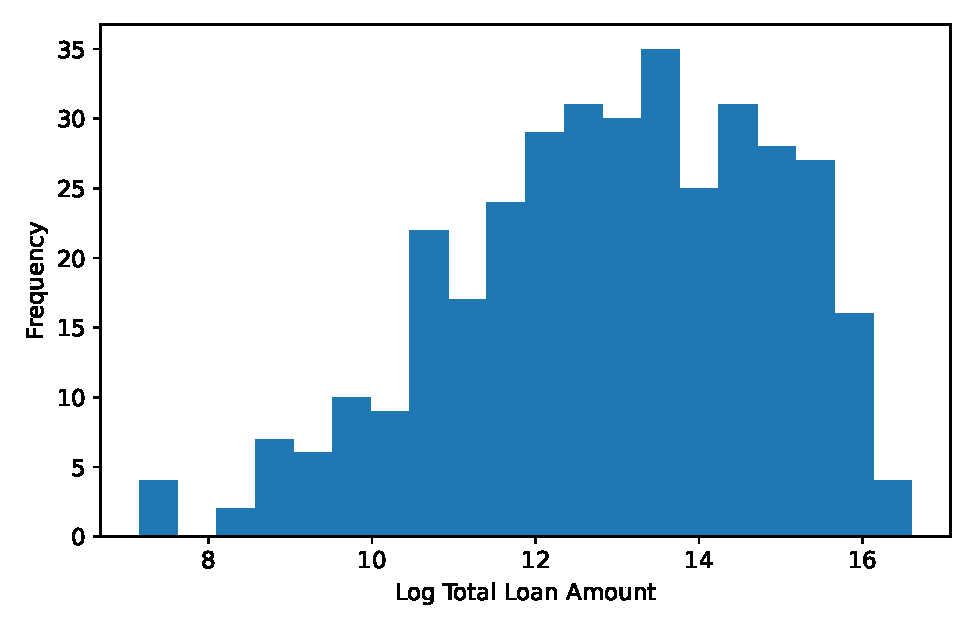
\includegraphics[width=0.75\textwidth]{figures/figure2_hist_lending.pdf}
\caption{Distribution of log total Kiva lending volume across country-years in the sample.}
\label{fig:fig2}
\end{figure}

\begin{figure}[htbp]
\centering
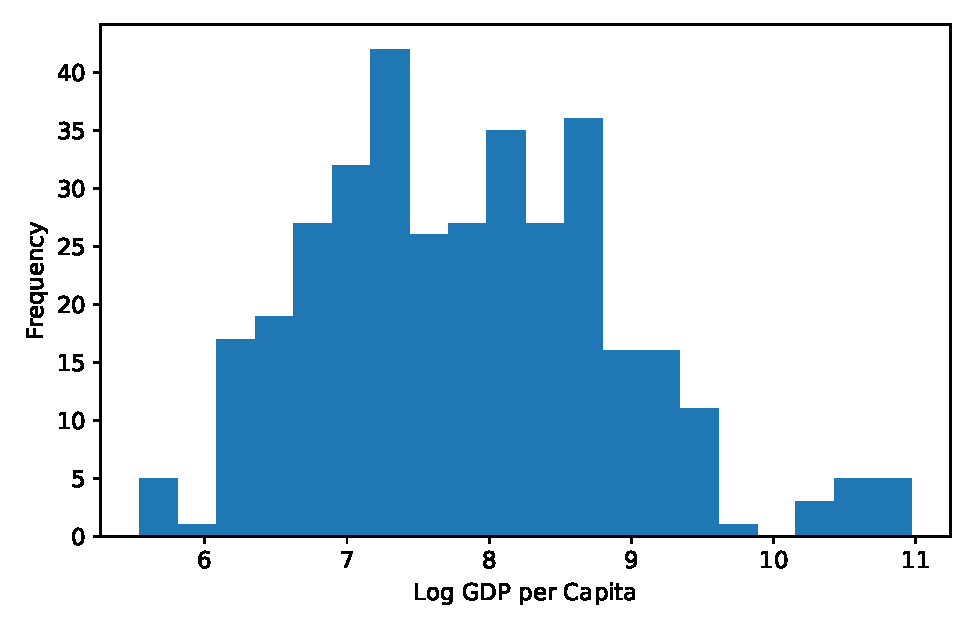
\includegraphics[width=0.75\textwidth]{figures/figure3_hist_gdp.pdf}
\caption{Distribution of log GDP per capita across country-years in the sample.}
\label{fig:fig3}
\end{figure}

\begin{figure}[htbp]
\centering
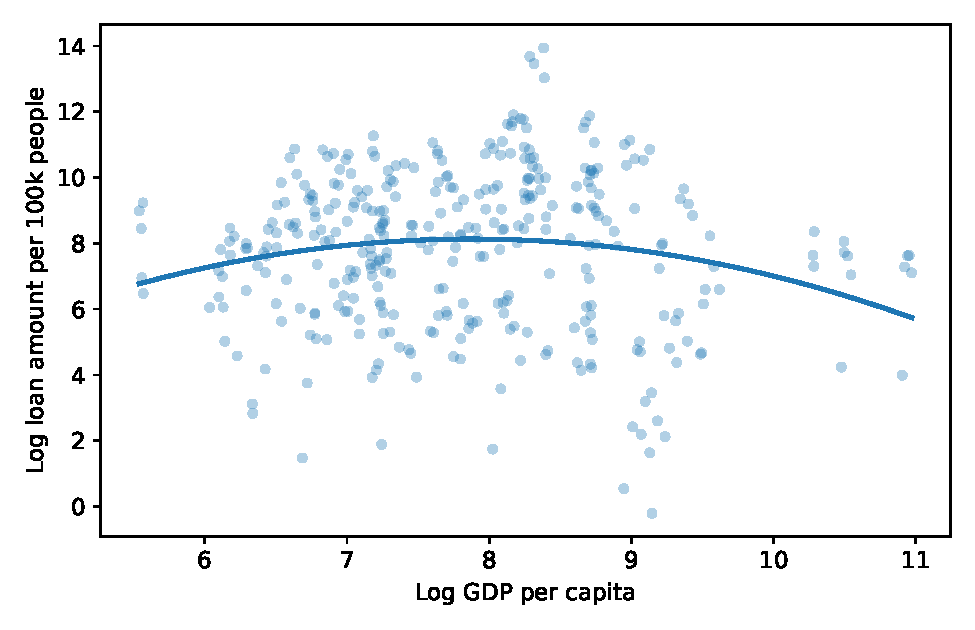
\includegraphics[width=0.75\textwidth]{figures/figure4_percapita.pdf}
\caption{Development and per-capita microfinance lending. Each point is one country-year; the
vertical axis is log Kiva loan volume per 100,000 people, with a quadratic fit overlaid.}
\label{fig:fig4}
\end{figure}

\begin{figure}[htbp]
\centering
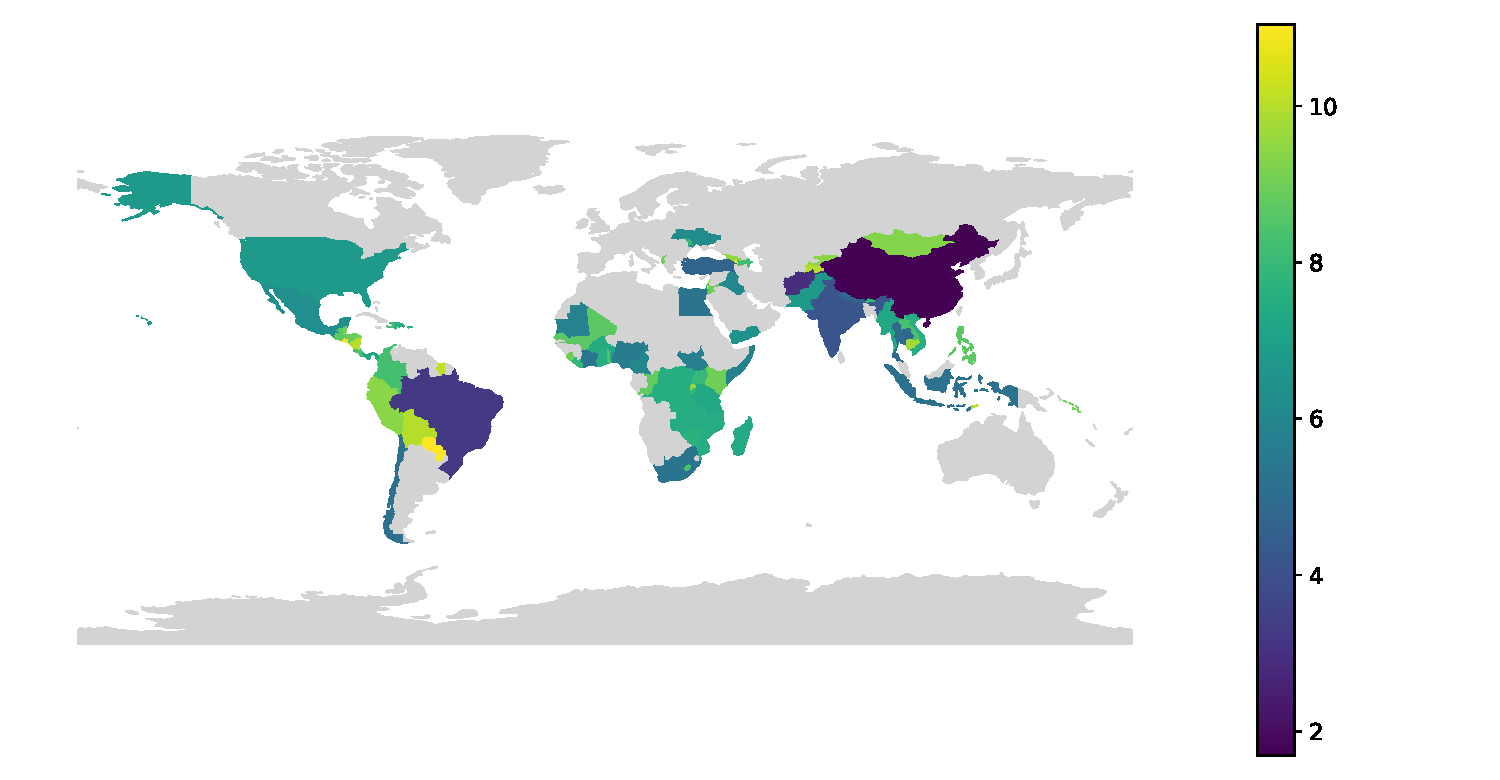
\includegraphics[width=0.72\textwidth]{figures/figure5_map_lending.pdf}
\caption{Average microfinance lending per 100,000 people by country, 2013--2017. Grey indicates no
Kiva-lending observations for that country in the panel.}
\label{fig:fig5}
\end{figure}

\begin{figure}[htbp]
\centering
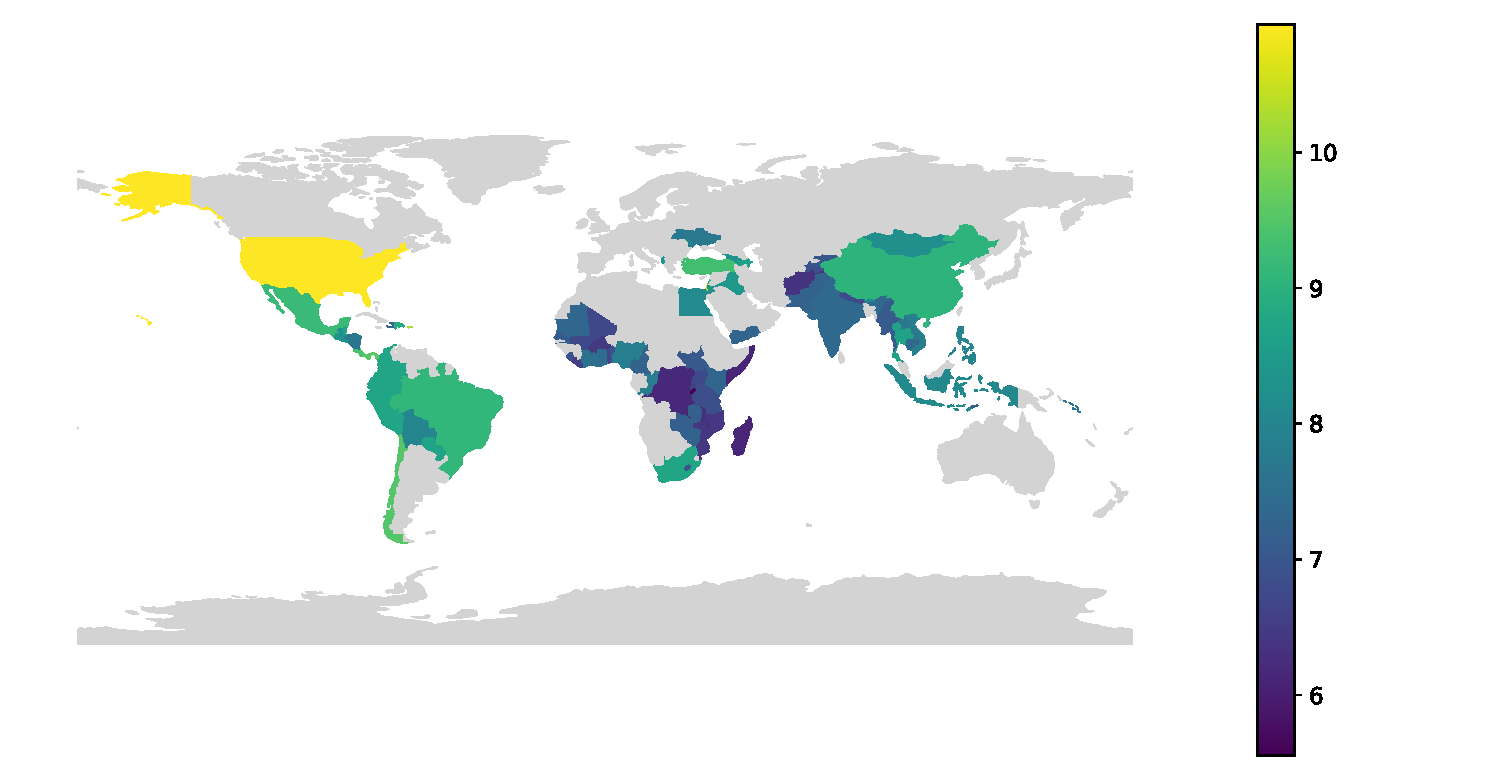
\includegraphics[width=0.72\textwidth]{figures/figure6_map_gdp.pdf}
\caption{Average log GDP per capita by country, 2013--2017.}
\label{fig:fig6}
\end{figure}

\begin{figure}[htbp]
\centering
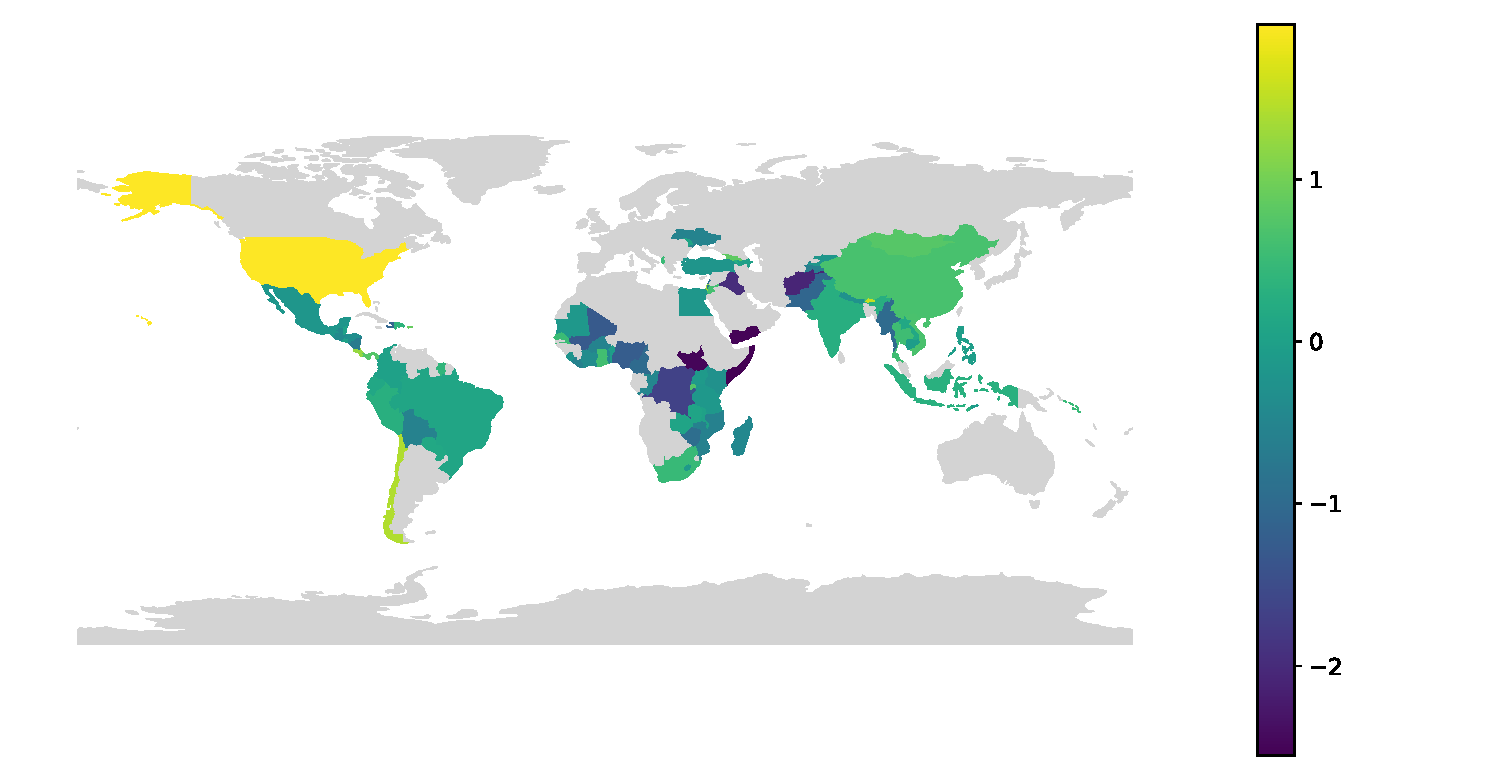
\includegraphics[width=0.72\textwidth]{figures/figure7_map_institutions.pdf}
\caption{Average institutional-quality index by country, 2013--2017.}
\label{fig:fig7}
\end{figure}

\section{Empirical Strategy}
\label{sec:strategy}

The regression analysis tests whether the descriptive patterns in Section~\ref{sec:descriptive}
survive formal specifications, at both the country-year and loan level. Two families of models are
estimated, one per outcome: \textbf{quantity models} (Section~\ref{sec:results-country}), dependent
variable log total lending volume, country-year panel, country-clustered standard errors; and
\textbf{size models} (Section~\ref{sec:results-loan}), dependent variable log loan amount, loan-level
panel, country-year-clustered standard errors (with a country-clustered robustness check in
Section~\ref{sec:robustness}). For each outcome, four linear/interaction specifications are estimated
--- a linear benchmark; linear plus institutions; adding year fixed effects; and adding an interaction
between development and institutional quality --- followed by four quadratic/robustness
specifications that add a squared development term (centered on the sample mean, to ease
interpretation of the linear term), then swap in year fixed effects and alternative institutional
measures. Both outcomes are tested with the same battery so that any divergence between them reflects
a difference in the underlying relationship, not a difference in specification.

Because a squared term can fit noise as readily as a genuine peak, the analysis treats
\emph{statistical significance of the quadratic term} as a necessary, not sufficient, criterion:
Section~\ref{sec:utest} adds a formal test of whether the implied curve actually turns within the
observed data range, applied uniformly to every shape claim in the paper, including the extensive
margin.

Two further design choices apply across every specification. First, log GDP per capita is centered on
its sample mean before squaring, so that the linear term in every quadratic specification can be read
directly as the slope of the curve at a representative point in the sample rather than at an
arbitrary and substantively meaningless zero. Second, every model is estimated with clustered standard
errors at the level appropriate to where the regressor of interest actually varies: country-clustered
for the country-year panel, since log GDP per capita is fixed within a country-year and repeated
observations of the same country over time are not independent draws; country-year-clustered for the
loan-level panel, since the same development regressors are repeated across every loan made in a given
country-year cell. Getting the clustering level wrong in either direction would overstate the precision
of the development coefficients specifically, which are the coefficients the paper's central claims
depend on --- so Section~\ref{sec:robustness} checks the loan-level choice directly against the
coarser alternative.

\section{Results}
\label{sec:results}

\subsection{Country-Year: Total Lending Volume}
\label{sec:results-country}

Table \ref{tab:table3} reports linear and interaction specifications for log total lending volume. The
coefficient on log GDP per capita is small, negative, and never statistically significant across the
linear models, which is itself informative because it suggests a one-directional specification is not
obviously the right functional form. Adding an interaction between development and institutional
quality, the delta-method marginal effect of development is negative at the 25th percentile, mean, and
75th percentile of institutional quality and is not statistically significant at any of them, so the
sample does not support a sign flip across institutional environments.

\begin{table}[htbp]
\centering
\caption{Country-Year: Linear and Interaction Specifications (Total Lending Volume)}
\label{tab:table3}
\begin{tabular}{lcccc}
\toprule
 & (1) & (2) & (3) & (4) \\
\midrule
Log GDP per capita & -0.060 & -0.181 & -0.179 & -0.130 \\
 & (0.150) & (0.158) & (0.169) & (0.165) \\
Institutional quality (PCA1) &  & 0.251 & 0.273 & 2.213 \\
 &  & (0.189) & (0.208) & (1.475) \\
Log population & 0.112 & 0.134 & 0.145 & 0.156 \\
 & (0.094) & (0.097) & (0.110) & (0.116) \\
Log GDP per capita $\times$ institutional quality &  &  &  & -0.252 \\
 &  &  &  & (0.195) \\
Constant & 11.605*** & 12.213*** & 9.801*** & 9.351*** \\
 & (2.068) & (1.968) & (2.171) & (2.400) \\
\midrule
Year fixed effects & No & No & Yes & Yes \\
Observations & 348 & 348 & 348 & 348 \\
\bottomrule
\end{tabular}
\par\smallskip\footnotesize Dependent variable: log total Kiva lending volume, country-year level. Standard errors in parentheses. Country-clustered standard errors. * $p<0.1$; ** $p<0.05$; *** $p<0.01$.
\end{table}

Table \ref{tab:table4} is the direct test of the middle-income-peak hypothesis at the country level,
and it does \textbf{not} support it. The squared development term is negative in all four
specifications, ranging from $-0.155$ to $-0.201$ (models 5--8), but is not statistically
distinguishable from zero in any of them ($p$ from 0.102 to 0.181, standard errors around 0.12--0.13).
The point estimate in the preferred specification implies a concave curve with a turning point at log
GDP per capita $\approx 7.456$ (about \$1,731 in constant 2015 USD), inside the sample range, but
because the quadratic coefficient itself is not significant, the data cannot reject a simpler
description --- a flat or monotonically declining relationship --- over the ``peak'' shape implied by
the point estimate. The linear component evaluated at the sample mean is also negative in every
specification, so the estimated relationship with development is a decline across most of the observed
income range, not a rise to a peak, and this pattern is stable across all three institutional-quality
measures and whether or not year fixed effects are included. \textbf{The country-level quadratic
pattern is therefore not treated as evidence of a middle-income peak in total lending volume;} the
more defensible summary is that total Kiva lending volume tends to be lower, not higher, in richer
countries within this sample, without strong evidence of a rise-then-fall shape.

\begin{table}[htbp]
\centering
\caption{Marginal Effect of Log GDP per Capita on Log Total Lending Volume (Model 4)}
\label{tab:table3b}
\resizebox{\textwidth}{!}{%
\begin{tabular}{lcccc}
\toprule
 & Institutional quality level & Marginal effect & SE & p-value \\
\midrule
25th percentile & -0.568 & 0.012 & 0.198 & 0.950 \\
Mean & -0.132 & -0.097 & 0.167 & 0.560 \\
75th percentile & 0.417 & -0.235 & 0.184 & 0.201 \\
\bottomrule
\end{tabular}%
}
\par\smallskip\footnotesize Delta-method marginal effects of log GDP per capita at percentiles of institutional quality, model (4).
\end{table}

\begin{table}[htbp]
\centering
\caption{Country-Year: Quadratic and Robustness Specifications (Total Lending Volume)}
\label{tab:table4}
\begin{tabular}{lcccc}
\toprule
 & (5) & (6) & (7) & (8) \\
\midrule
Log GDP per capita (centered) & -0.117 & -0.111 & -0.121 & -0.162 \\
 & (0.153) & (0.165) & (0.167) & (0.237) \\
Log GDP per capita\textsuperscript{2} (centered) & -0.155 & -0.168 & -0.170 & -0.201 \\
 & (0.116) & (0.125) & (0.125) & (0.123) \\
Institutional quality (PCA1) & 0.274 & 0.297 &  &  \\
 & (0.185) & (0.204) &  &  \\
Institutional quality index &  &  & 0.338 &  \\
 &  &  & (0.224) &  \\
Financial access index &  &  &  & 0.305 \\
 &  &  &  & (0.286) \\
Log population & 0.154 & 0.166 & 0.161 & 0.114 \\
 & (0.100) & (0.114) & (0.112) & (0.105) \\
Constant & 10.655*** & 8.233*** & 8.318*** & 9.034*** \\
 & (1.663) & (1.899) & (1.870) & (1.739) \\
\midrule
Year fixed effects & No & Yes & Yes & Yes \\
Observations & 348 & 348 & 348 & 319 \\
\bottomrule
\end{tabular}
\par\smallskip\footnotesize Dependent variable: log total Kiva lending volume, country-year level. Log GDP per capita is centered. Standard errors in parentheses. Country-clustered standard errors. * $p<0.1$; ** $p<0.05$; *** $p<0.01$.
\end{table}

Year fixed effects in the preferred specification rise from the omitted 2013 baseline by roughly 2.3
to 2.9 log points in 2014--2017, with no further monotonic increase after 2014 --- consistent with
Kiva's total lending volume genuinely expanding over this period (total dollar volume rises from about
\$133.0M in 2013 to \$175.6M in 2017, per Table \ref{tab:tableA1}) rather than with a
sample-composition change, since country coverage grows far less (74 to 76 countries) than dollar
volume does. This supports reading the year effects as a platform-growth control rather than as
evidence bearing on the development--lending relationship itself.

\subsection{Loan Level: Individual Loan Size}
\label{sec:results-loan}

The country-year regressions preserve the main macroeconomic story, but the number of observations is
mechanically limited by the number of countries and years (348 in the regression sample). To test the
same nonlinearity question on the intensive margin, the same eight specifications are estimated at the
\textbf{loan level}, using 917,955 individual Kiva loans merged to the same macro covariates. The
dependent variable becomes log loan amount, so these coefficients describe how country-year
development conditions are associated with the \emph{size of a typical loan}, not aggregate lending
volume --- a distinct question, not a higher-powered re-estimate of Section~\ref{sec:results-country}.
Because development varies at the country-year level while loan size varies at the loan level, the
main specifications use country-year clustered standard errors, with a country-clustered version
reported as a robustness check.

The linear and interaction specifications (Table \ref{tab:table5}, Appendix) mirror
Table \ref{tab:table3}: the development coefficient is negative, and the delta-method marginal effect
from the interaction specification is negative across the range of institutional quality, though with
far tighter standard errors given the much larger sample. With roughly 900,000 loans rather than 348
country-years, these models have far more power to detect a nonlinear pattern if one exists. The
squared development term is \textbf{positive and statistically
significant at the 1\% level} ($0.245$, $p<0.001$, preferred specification) in every quadratic
specification. This is a \textbf{U-shape, not an inverted-U}: individual loan size is estimated to
fall as development rises from the low end of the sample, reach a minimum, and then rise again at
higher development levels --- the opposite sign from the (statistically insignificant) country-level
pattern. This is not a contradiction, because the two outcomes measure different objects: a country
can plausibly receive less total lending as it develops (fewer, larger loans crowd out many small
ones, and formal banking substitutes for Kiva overall) while the loans that \emph{are} still made
through Kiva get smaller in lower-middle income settings --- where Kiva serves a high volume of very
small borrowers --- before rising again as remaining Kiva borrowers in richer countries use it for
larger, more bank-like loan sizes. Sections~\ref{sec:results-country} and \ref{sec:results-loan}
should therefore be read as two separate, both well-supported findings about different margins of
microfinance activity, not as two tests of one shared hypothesis.

\begin{table}[htbp]
\centering
\caption{Marginal Effect of Log GDP per Capita on Log Loan Size (Model 4, Loan Level)}
\label{tab:table5b}
\resizebox{\textwidth}{!}{%
\begin{tabular}{lcccc}
\toprule
 & Institutional quality level & Marginal effect & SE & p-value \\
\midrule
25th percentile & -0.290 & 0.189 & 0.057 & 0.001 \\
Mean & -0.147 & 0.225 & 0.055 & 0.000 \\
75th percentile & -0.012 & 0.259 & 0.054 & 0.000 \\
\bottomrule
\end{tabular}%
}
\par\smallskip\footnotesize Delta-method marginal effects of log GDP per capita at percentiles of institutional quality, loan-level model (4).
\end{table}

\begin{table}[htbp]
\centering
\caption{Loan-Level: Quadratic and Robustness Specifications (Loan Size)}
\label{tab:table6}
\begin{tabular}{lcccc}
\toprule
 & (5) & (6) & (7) & (8) \\
\midrule
Log GDP per capita (centered) & 0.201*** & 0.206*** & 0.209*** & 0.166*** \\
 & (0.050) & (0.049) & (0.050) & (0.064) \\
Log GDP per capita\textsuperscript{2} (centered) & 0.245*** & 0.245*** & 0.245*** & 0.211*** \\
 & (0.030) & (0.028) & (0.028) & (0.050) \\
Institutional quality (PCA1) & -0.091 & -0.094 &  &  \\
 & (0.066) & (0.066) &  &  \\
Institutional quality index &  &  & -0.110 &  \\
 &  &  & (0.075) &  \\
Financial access index &  &  &  & 0.043 \\
 &  &  &  & (0.082) \\
Log population & -0.207*** & -0.204*** & -0.201*** & -0.203*** \\
 & (0.028) & (0.027) & (0.026) & (0.028) \\
Constant & 9.713*** & 9.764*** & 9.718*** & 9.778*** \\
 & (0.455) & (0.451) & (0.445) & (0.473) \\
\midrule
Year fixed effects & No & Yes & Yes & Yes \\
Observations & 913,128 & 913,128 & 913,128 & 891,246 \\
\bottomrule
\end{tabular}
\par\smallskip\footnotesize Dependent variable: log individual loan amount. Log GDP per capita is centered. Standard errors in parentheses. Country-year-clustered standard errors. * $p<0.1$; ** $p<0.05$; *** $p<0.01$.
\end{table}

\subsection{Two Margins: Extensive versus Intensive}
\label{sec:results-extensive}

Sections~\ref{sec:results-country} and \ref{sec:results-loan} both condition on Kiva already lending
in a country-year: countries with no Kiva presence simply do not appear in the country-year panel at
all. That means Table \ref{tab:table4}'s insignificant quadratic term cannot distinguish two very
different stories: development has no nonlinear relationship with Kiva activity at any margin, or
development \emph{does} have a nonlinear relationship with \textbf{whether Kiva is active in a
country at all} (the extensive margin), but that pattern is invisible in Table \ref{tab:table4}
because the regression only ever sees countries where the answer is already yes.

To test this, a \textbf{global country-year panel that includes true zeros} is built: every economy
with World Bank GDP-per-capita and population data for 2013--2017 is outer-merged with Kiva
country-year loan totals built directly from raw loan-posting data, so that country-years with no
matching Kiva loans get a lending total of zero and a Kiva-active indicator of zero rather than being
dropped. Country codes are harmonized to a common three-letter standard for the merge, since Kiva's own
loan records use two-letter codes while the World Bank series use three-letter codes; this resolves
cleanly for every one of Kiva's 90 country codes, including territory-style codes such as the one used
for Kosovo. The World Development Indicators classify 217 economies as actual countries, excluding
regional and income-group aggregates such as ``Sub-Saharan Africa.'' Of the resulting 1,085 candidate
country-year cells, 65 are dropped for missing GDP per capita or population (mostly small territories
and a few years of state fragility), leaving \textbf{1,020 country-years covering 206 countries}, of
which \textbf{374 (36.7\%) are Kiva-active}.
Because institutional and financial-access variables are only available for the roughly 90--96
countries Kiva already covers, they are heavily missing in the global sample and are not used as
controls in the global regressions; institutional quality is reintroduced only in the Kiva-only
intensive-margin column, where coverage is adequate.

Two models are estimated on this global panel. The \textbf{extensive margin} is modeled with
\textbf{Logit} (country-clustered standard errors, reporting both coefficients and average marginal
effects). The \textbf{intensive margin} is modeled with \textbf{PPML} (Poisson pseudo-maximum-
likelihood; \citealp{santossilva2006}), because the outcome now includes true zeros and a log-linear
OLS model is not an option --- dropping zeros would simply reproduce Section~\ref{sec:results-country}'s
selected sample. PPML is estimated both on the full global sample including zeros and on the Kiva-only
subsample, so the same functional form can be compared with and without the zero-lending
country-years.

\begin{table}[htbp]
\centering
\caption{Extensive Margin: Logit Coefficients and Average Marginal Effects}
\label{tab:table8}
\begin{tabular}{lcc}
\toprule
 & Coefficient & Average marginal effect \\
\midrule
Log GDP per capita (centered) & -1.026*** & -0.157*** \\
 & (0.204) & (0.024) \\
Log GDP per capita\textsuperscript{2} (centered) & -0.260** & -0.040** \\
 & (0.114) & (0.017) \\
Log population & 0.399*** & 0.061*** \\
 & (0.086) & (0.011) \\
\midrule
Year fixed effects & Yes & Yes \\
Observations & 1,020 & 1,020 \\
Pseudo $R^2$ & 0.301 & \\
\bottomrule
\end{tabular}
\par\smallskip\footnotesize Dependent variable: indicator for Kiva active in a country-year, global panel including zero-lending country-years. Country-clustered standard errors in parentheses. Log GDP per capita is centered. * $p<0.1$; ** $p<0.05$; *** $p<0.01$.
\end{table}

\begin{table}[htbp]
\centering
\caption{Two Margins: Logit (Extensive) vs. PPML (Intensive), Development Terms}
\label{tab:table9}
\resizebox{\textwidth}{!}{%
\begin{tabular}{lccccccc}
\toprule
Covariate & Logit coef. & Logit p & Logit AME & PPML (global) coef. & PPML (global) p & PPML (Kiva-only) coef. & PPML (Kiva-only) p \\
\midrule
Log GDP per capita (centered) & -1.0265 & 0.0000 & -0.1569 & -0.5407 & 0.1611 & -0.0055 & 0.9808 \\
Log GDP per capita\textsuperscript{2} (centered) & -0.2603 & 0.0226 & -0.0398 & -0.2318 & 0.2417 & -0.0698 & 0.5300 \\
\bottomrule
\end{tabular}%
}
\par\smallskip\footnotesize Logit: global panel including zero-lending country-years, country-clustered SE. PPML (global): same sample; PPML (Kiva-only): restricted to Kiva-active country-years. All models include year fixed effects and log population; PPML (Kiva-only) also includes institutional quality.
\end{table}

\begin{figure}[htbp]
\centering
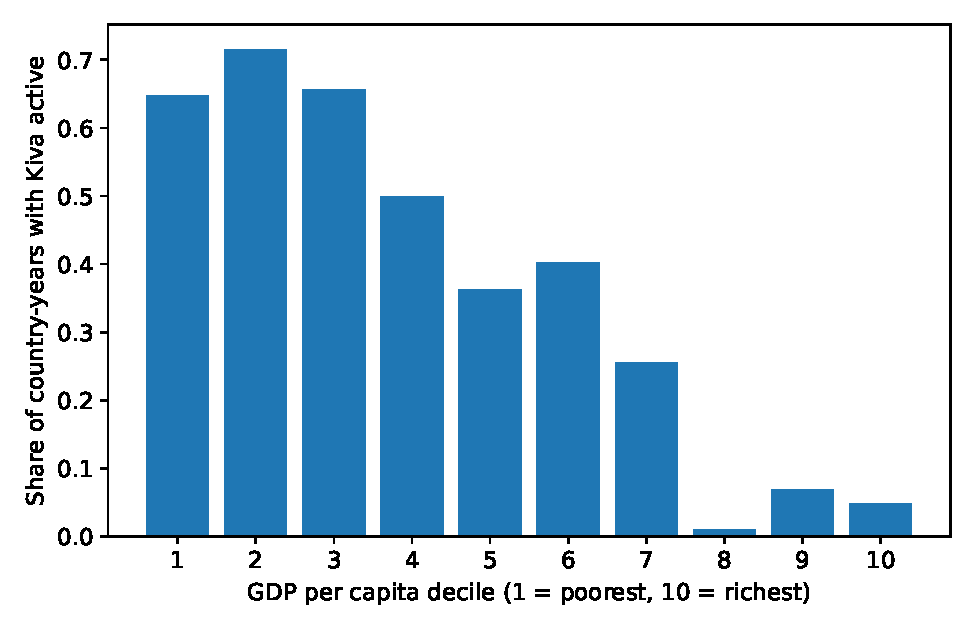
\includegraphics[width=0.75\textwidth]{figures/figure8_entry_by_decile.pdf}
\caption{Share of country-years with Kiva active, by decile of log GDP per capita (1 = poorest
decile, 10 = richest decile), global panel including zero-lending country-years.}
\label{fig:fig8}
\end{figure}

Table \ref{tab:table9} (with full Logit coefficients and average marginal effects in Table
\ref{tab:table8}) shows where the strongest evidence for development-related nonlinearity lives, with
an important qualification from the formal test in Section~\ref{sec:utest}. The \textbf{extensive
margin is significantly concave}: the Logit quadratic term is negative and significant (coefficient
$-0.260$, $p=0.023$; average marginal effect $-0.040$, $p=0.018$), and Figure~\ref{fig:fig8} shows the
pattern directly in the raw data --- Kiva's entry rate is roughly two-thirds across the poorest three
deciles, falls to half by the fourth decile, and declines steeply to between 1\% and 7\% in the top
three deciles. The implied turning point is at log GDP per capita $\approx 6.79$ (about \$893 in
constant 2015 USD), very close to the low end of the sample. Applying the same Lind--Mehlum test used
for the other margins (Section~\ref{sec:utest}), the high-end decline is unambiguous but the low-end
\emph{rise} is not individually significant ($t=1.07$, one-sided $p=0.143$), so the data confirm
concavity and a steep decline with development, not a completed rise-then-fall within the observed
range.

The \textbf{intensive margin does not show this pattern, whether or not zeros are included.} PPML on
the full global sample gives a quadratic coefficient of $-0.232$ ($p=0.242$); PPML restricted to the
369 (of 374) Kiva-active country-years with complete institutional controls gives $-0.070$
($p=0.530$). Both are statistically indistinguishable from zero, echoing the OLS-in-logs result in
Table \ref{tab:table4} even though PPML uses a completely different estimator and, in the global
specification, a completely different zero-inclusive sample. Development therefore matters most
visibly for \emph{whether} Kiva operates in a country, with entry probability significantly concave in
income and falling steeply as countries develop; but that is not the same as a confirmed inverted-U,
because the initial rise at the very bottom of the income distribution cannot be statistically
distinguished from a flat start. The three-margin picture is therefore: (1) whether Kiva enters a
country --- significantly concave, steeply declining, peak unconfirmed; (2) how much a country
receives in total, conditional on entry --- flat/declining, not significant; (3) how large an
individual loan is --- U-shaped, significant and formally confirmed. These are three distinct
empirical objects, and the original middle-income-peak intuition survives, at most, in weakened form
at the first of them.

\subsection{Formal Test for Nonlinearity: The Lind--Mehlum U-Test}
\label{sec:utest}

Throughout Sections~\ref{sec:results-country}--\ref{sec:results-extensive}, whether the quadratic term
is statistically significant has been the main criterion for taking a nonlinear pattern seriously.
That criterion is necessary but not sufficient: a significant quadratic coefficient does not by itself
guarantee that the curve actually turns within the observed data range, because a significant
coefficient combined with a turning point far outside the sample would imply an essentially monotonic
relationship over the range actually observed. \citet{lindmehlum2010} formalize the correct test: a
genuine U-shape (or inverted-U) requires that the slope of the curve be significantly negative
(positive) at the low end of the sample and significantly positive (negative) at the high end,
evaluated at the sample's actual minimum and maximum of $X$, not just that the quadratic coefficient
differs from zero at the sample mean.

Concretely, for a fitted quadratic $\hat{y} = \hat\beta_0 + \hat\beta_1 x + \hat\beta_2 x^2 +
\text{controls}$, the slope at any point is $\hat\beta_1 + 2\hat\beta_2 x$. This slope is computed at
$x_{\min}$ and $x_{\max}$ (the sample extremes of centered log GDP per capita), with its standard
error obtained via the delta method,
\begin{equation}
\label{eq:delta-se}
\mathrm{SE}\big(\hat\beta_1 + 2\hat\beta_2 x\big) = \sqrt{\mathrm{Var}(\hat\beta_1) +
(2x)^2\,\mathrm{Var}(\hat\beta_2) + 2(2x)\,\mathrm{Cov}(\hat\beta_1,\hat\beta_2)},
\end{equation}
using each model's full clustered covariance matrix so the covariance term is not assumed away, and
both slopes are tested individually. Following Lind and Mehlum's intersection-union logic (closely
related to \citealp{sasabuchi1980}), the overall test statistic is the \textbf{weaker of the two
individual $t$-statistics} in absolute value: the shape is confirmed only if both ends pass, so the
binding constraint is whichever end is less significant. A \citet{fieller1954} confidence interval is
also reported for the turning point $x_0 = -\hat\beta_1/(2\hat\beta_2)$, which correctly accounts for
$x_0$ being a ratio of two estimated, correlated coefficients; if the quadratic term is not precisely
estimated relative to the critical value, the Fieller interval is unbounded, which is itself
informative.

This test is applied to all three shape claims in the paper: \textbf{m6} (country-year, total lending
volume), \textbf{lm6} (loan-level, individual loan size), and the \textbf{extensive-margin Logit}
(Section~\ref{sec:results-extensive}), the last evaluated on the linear-index (log-odds) scale where
the quadratic functional form lives.

\begin{table}[htbp]
\centering
\caption{Lind--Mehlum (2010) U-Test: m6, lm6, and the Extensive-Margin Logit}
\label{tab:table10}
\resizebox{\textwidth}{!}{%
\begin{tabular}{lccccccc}
\toprule
Model & Slope (low) & $t$ (low) & Slope (high) & $t$ (high) & U-test $p$ & Confirmed? & Fieller 95\% CI \\
\midrule
m6 (country-year, volume) & 0.659 & 1.080 & -1.162 & -1.478 & 0.140 & No & Unbounded \\
lm6 (loan-level, size) & -0.893 & -5.752 & 1.766 & 10.954 & 0.000 & Yes & [-0.730, -0.198] \\
Logit (global, extensive margin) & 0.654 & 1.065 & -2.742 & -3.028 & 0.143 & No & [-10.384, -1.216] \\
\bottomrule
\end{tabular}%
}
\par\smallskip\footnotesize Slopes evaluated at the sample minimum and maximum of (centered) log GDP per capita, with delta-method standard errors using each model's full clustered covariance matrix. The U-test statistic is the weaker of the two end $t$-statistics (one-sided); shape is confirmed only if both ends are individually significant at the 5\% level with opposite-signed slopes. The Logit row is evaluated on the linear-index (log-odds) scale.
\end{table}

Table \ref{tab:table10} confirms, formally, what the p-value-only
discussion above already suggested informally. For \textbf{m6}, the slope at the low end of the sample
is positive but only $t\approx1.08$, well short of conventional significance, so the weaker-end test
statistic fails decisively (one-sided $p\approx0.140$), and the Fieller confidence interval for the
turning point is \textbf{unbounded} --- the data are consistent with a turning point essentially
anywhere, including outside the observed range. This is independent confirmation that the
country-level ``peak'' should not be treated as an established finding.

For \textbf{lm6}, the result is the opposite in every respect: the slope is significantly negative at
the low end ($t\approx-5.75$) and significantly positive at the high end ($t\approx10.95$), both
comfortably clearing the bar, so the U-test \textbf{confirms} the shape (one-sided $p<0.001$). The
Fieller confidence interval for the turning point is tight and lies well inside the sample range, at
roughly log GDP per capita $\approx7.05$--$7.59$ (about \$1,150--\$1,970 in constant 2015 USD),
bracketing the point estimate of $\approx7.36$ (\$1,577). This is the formal, quantitative basis for
treating the loan-level U-shape as the paper's central confirmed nonlinear finding and the
country-level curvature as unsupported.

For the \textbf{extensive-margin Logit}, the test delivers a split verdict. The high-end slope is
strongly negative and individually significant ($t=-3.03$), confirming the steep decline in entry
probability among richer countries. But the low-end slope, while positive, is not individually
significant ($t=1.07$, one-sided $p=0.143$), so the intersection-union test fails and the inverted-U is
not formally confirmed: the data cannot rule out that entry probability is simply flat at the very
bottom of the income distribution before declining. This is the same discipline that the country-level
curvature was held to, applied symmetrically to the paper's most favorable-looking result: the
extensive margin is reported as significant concavity with a steep decline, not as an established
peak.

\section{Robustness}
\label{sec:robustness}

\subsection{Clustering Choice}

The loan-level main specifications cluster standard errors at the country-year level, because the
country-year development regressors are mechanically repeated within every country-year cell of loans,
so treating each loan as an independent observation for inference would overstate precision. As a
direct check on that choice, the preferred loan-level specification is re-estimated with standard
errors clustered at the coarser country level instead (Table \ref{tab:table7}, Appendix). The standard
errors on the development terms are of similar magnitude under both choices, so the significance of the
loan-level quadratic term is not an artifact of the finer country-year clustering.

\subsection{Sample Period: Does Including 2013 Matter?}

Section~\ref{sec:sample-period} concluded that 2013 is a complete year of genuine, if smaller, Kiva
activity and should be kept in the main sample. As a direct check on that judgment call, the preferred
quadratic specifications --- \textbf{m6} (country-year, total volume) and \textbf{lm6} (loan-level, loan
size) --- are re-estimated on the 2014--2017 subsample only, dropping 2013 entirely, and the development
terms are compared side by side with the full-sample results (Table \ref{tab:table11}).

\begin{table}[htbp]
\centering
\caption{Sample-Period Robustness: Full Sample vs. 2014--2017 Only}
\label{tab:table11}
\resizebox{\textwidth}{!}{%
\begin{tabular}{lccccc}
\toprule
Specification & Linear coef. & $p$ & Quadratic coef. & $p$ (sq.) & N \\
\midrule
m6, full sample (2013-2017) & -0.1106 & 0.5018 & -0.1676 & 0.1795 & 348.0000 \\
m6, 2014-2017 only & -0.0947 & 0.5945 & -0.1760 & 0.1594 & 294.0000 \\
lm6, full sample (2013-2017) & 0.2055 & 0.0000 & 0.2447 & 0.0000 & 913128.0000 \\
lm6, 2014-2017 only & 0.1874 & 0.0008 & 0.2456 & 0.0000 & 776306.0000 \\
\bottomrule
\end{tabular}%
}
\par\smallskip\footnotesize m6: country-year volume model; lm6: loan-level size model, both with year fixed effects.
\end{table}

Both conclusions are unchanged: at the country level, the quadratic term
moves from $-0.168$ ($p=0.179$, full sample) to $-0.176$ ($p=0.159$, 2014--2017 only) --- still
negative, still far from significant; at the loan level, the quadratic term is virtually identical
($0.245$, $p<0.001$ in both the full sample and the 2014--2017-only subsample), with the linear term
also stable ($0.206$ versus $0.187$). The paper's two central conclusions do not depend on the
decision to keep 2013 in the sample.

\subsection{Loan-Level Robustness: Alternative Specifications of the Size Margin}

The loan-level U-shape is the paper's central confirmed nonlinear finding, so it is worth
stress-testing directly rather than only checking the clustering choice and the sample period above.
The preferred loan-level specification is re-estimated under three additional variants (Table
\ref{tab:table12}), with the formal shape test applied to each (Table \ref{tab:table13}): excluding the
United States, since US-based Kiva loans are a qualitatively different product (small-business loans in
a high-income economy) rather than the poverty-lending use case the rest of the panel represents, and
could be driving the ``rises again'' half of the U-shape by themselves; a relative-loan-size measure
that deflates the nominal loan amount by local GDP per capita, to check whether the U-shape partly
reflects price- or income-level scaling rather than a real change in typical loan size; and sector fixed
effects, since Kiva's raw data classify every loan into one of fifteen sectors and richer and poorer
countries in the sample could differ systematically in which sectors are active, which would make an
apparent size U-shape partly a compositional artifact rather than a within-sector pattern.

\begin{table}[htbp]
\centering
\caption{Loan-Level Robustness: lm6 Under Four Specifications}
\label{tab:table12}
\resizebox{\textwidth}{!}{%
\begin{tabular}{lccccc}
\toprule
Specification & Linear coef. & $p$ & Quadratic coef. & $p$ (sq.) & N \\
\midrule
(1) Baseline (lm6) & 0.2055 & 0.0000 & 0.2447 & 0.0000 & 913128.0000 \\
(2) Excluding US & 0.2289 & 0.0000 & 0.3322 & 0.0000 & 904855.0000 \\
(3) Relative loan size & -0.7945 & 0.0000 & 0.2447 & 0.0000 & 913128.0000 \\
(4) Sector fixed effects & 0.1925 & 0.0001 & 0.2340 & 0.0000 & 913128.0000 \\
\bottomrule
\end{tabular}%
}
\par\smallskip\footnotesize (3) Relative loan size regresses log(loan amount / local GDP per capita) on the same controls; because log GDP per capita already enters linearly, this reproduces (1) by a Frisch--Waugh--Lovell identity and is not independently informative about curvature (see text). All columns use country-year-clustered standard errors.
\end{table}

\begin{table}[htbp]
\centering
\caption{Lind--Mehlum U-Test Applied to All Four Loan-Level Robustness Variants}
\label{tab:table13}
\resizebox{\textwidth}{!}{%
\begin{tabular}{lcccc}
\toprule
Specification & $t$, low end & $t$, high end & U-test $p$ & Shape confirmed \\
\midrule
(1) Baseline (lm6) & -5.752 & 10.954 & 0.000 & Yes \\
(2) Excluding US & -4.868 & 7.129 & 0.000 & Yes \\
(3) Relative loan size & -12.194 & 4.750 & 0.000 & Yes \\
(4) Sector fixed effects & -5.650 & 11.071 & 0.000 & Yes \\
\bottomrule
\end{tabular}%
}
\par\smallskip\footnotesize One-sided U-test statistics for each column of Table \ref{tab:table12}.
\end{table}

\textbf{Excluding the United States} barely matters and if anything
strengthens the pattern: US-based loans are only 0.9\% of this sample, and the quadratic term rises
slightly to $0.332$ (still $p<0.001$) once the US is dropped, so the ``richer countries get larger
loans again'' half of the U-shape is not a US-specific artifact. \textbf{Relative loan size} (loan
amount deflated by local GDP per capita) requires a genuine caveat: the quadratic coefficient in this
column is numerically identical to the baseline's ($0.245$ in both, to three decimal places) because
$\log(\text{loan amount}/\text{GDP per capita})$ is algebraically $\log(\text{loan amount}) -
\log(\text{GDP per capita})$, and log GDP per capita is already the model's own linear regressor. By
the Frisch--Waugh--Lovell theorem, subtracting a variable already in the design matrix from the
dependent variable can only shift that variable's own coefficient (here, by exactly $-1$) and leaves
every other coefficient, including the quadratic term, mechanically unchanged; this specification, as
given, cannot actually test whether the nominal-dollar U-shape survives deflating by local price
levels, since it is guaranteed to reproduce the original quadratic term regardless of the true
data-generating process. A supplementary check that removes the self-cancelling linear control shows
the quadratic term \textbf{attenuates but survives}: $0.148$ (down from $0.245$), still significant at
$p=0.002$. The honest reading is that some, but probably not all, of the nominal-dollar U-shape's
magnitude reflects local price- or income-level scaling, while a statistically significant U-shaped
pattern in the deflated measure remains. \textbf{Sector fixed effects} leave the quadratic term
essentially unchanged ($0.234$ versus $0.245$ in the baseline, both $p<0.001$), so compositional
shifts across Kiva's fifteen lending sectors are not driving the result. Table \ref{tab:table13}
confirms with the formal shape test that all four variants pass decisively, including the relative-size
column for the mechanical reason just explained, which is why that particular ``pass'' should not be
read as additional independent evidence beyond what the supplementary, linear-control-free check
already provides.

\section{Limitations}
\label{sec:limitations}

The results above are subject to several limitations that bear directly on how much weight to place on
each of the three margins. Some are fully resolved by the paper's own design choices (building the
global zero-inclusive panel, running the formal shape test uniformly); others are only partially
addressed and are flagged as such below, rather than smoothed over.

\textbf{Sample selection (partially addressed).} The country-year and loan-level panels
(Sections~\ref{sec:results-country}--\ref{sec:results-loan}) cover only the countries in which Kiva
was already active between 2013 and 2017; whether Kiva enters a country at all is itself a decision
shaped by local infrastructure, regulation, and partner-organization availability, and that entry
decision is not modeled in those two panels. Section~\ref{sec:results-extensive} directly addresses
part of this by building a global panel that includes zero-lending country-years and modeling entry
with a Logit, but it still cannot say \emph{why} Kiva enters some countries and not others beyond the
reduced-form relationship with GDP per capita and population.

\textbf{Zero-lending country-years and the log transform (addressed at the country level, not the
loan level).} Log total lending volume and log loan size are well-defined and strictly positive for
every row in their respective panels, since there are no zero-loan country-years or zero-dollar loans
within the Kiva-only samples. Section~\ref{sec:results-extensive}'s global panel resolves this at the
country level by including true zeros and modeling them with a Logit rather than dropping them; there
is no loan-level analogue of this concern, since individual realized loans are by definition non-zero.

\textbf{Short panel.} The panel spans only five years (2013--2017). Some of the observed variation may
reflect the global expansion of the Kiva platform over this period rather than only structural
differences across countries; Section~\ref{sec:sample-period} checks that 2013 is not a partial or
incomplete year and Section~\ref{sec:robustness} confirms the main results are unchanged if 2013 is
dropped, but the panel remains short relative to typical macro panels, and year fixed effects only
partially absorb platform-growth effects that may themselves vary by country.

\textbf{Price-level and currency-conversion effects (partially addressed).}
Section~\ref{sec:robustness} shows that a naive test of whether the loan-level U-shape survives
deflating by local GDP per capita is mechanically guaranteed to reproduce the original result, and that
a corrected version of the same test shows the U-shape attenuates but remains significant. This
suggests part, but apparently not all, of the nominal-dollar loan-size U-shape reflects local
price-level scaling rather than a real change in relative loan size --- a distinction future work could
pursue further with a proper purchasing-power-parity or local-currency deflator.

\textbf{Descriptive, not causal.} All specifications are estimated by OLS, Logit, or PPML on
observational data. Development, institutional quality, and Kiva lending are jointly determined by
many unobserved factors, so the coefficients reported here should be read as conditional associations,
not treatment effects.

\section{Conclusion}
\label{sec:conclusion}

This paper set out to test whether Kiva microfinance lending activity follows an inverted-U
relationship with economic development, peaking in lower-middle income countries. The country-year
evidence does not support that hypothesis: the quadratic term is negative but statistically
indistinguishable from zero in all four specifications ($p>0.10$), and the linear component is
negative on average, so the more defensible reading is that \textbf{total lending volume tends to
decline with development} across most of the sample, without strong evidence of a rise-then-fall
shape. The formal Lind--Mehlum test confirms this is not just a significance-testing artifact: the
slope at the low end of the sample is not even individually significant ($t\approx1.08$), and the
Fieller confidence interval for the implied turning point is unbounded.

At the loan level, a different and much better-supported pattern emerges: the quadratic term is
\textbf{positive and significant at the 1\% level}, implying that individual loan size follows a
\textbf{U-shape} --- falling and then rising with development --- the opposite sign from the
(insignificant) country-level curvature. The formal test confirms this shape decisively, with a Fieller
turning-point interval of roughly \$1,150--\$1,970 that lies comfortably inside the sample range, and
this survives excluding the US, sector fixed effects, and (with attenuated but still significant
magnitude once a mechanical cancellation is correctly accounted for) deflating by local price levels.

A third margin resolves an ambiguity in the first two: because the country-year panel only contains
country-years where Kiva was already active, it cannot distinguish ``no nonlinearity anywhere'' from
``the nonlinearity is in whether Kiva enters a country at all.'' Building a global panel that includes
true zero-lending country-years and estimating a Logit for Kiva's extensive margin shows
\textbf{significant concavity with a steep decline}: the probability that Kiva is active in a country
is highest among the poorest deciles and falls to near zero among the richest countries, though the
initial rise at the very bottom fails the formal low-end slope test, so a completed inverted-U is not
established. PPML on total lending volume, both including zeros and restricted to Kiva-active
country-years, shows no such pattern, consistent with the OLS-in-logs result.

Because total volume, Kiva presence, and loan size measure three different objects --- aggregate
country-level volume, whether Kiva operates in a country at all, and the size of a single realized
loan --- these are not competing estimates of one underlying relationship. They are three distinct
findings about three different margins of microfinance activity:
\begin{enumerate}
\item \textbf{Extensive margin (country level, whether Kiva is active at all):} significantly
  concave --- entry probability declines steeply with development; the raw-data peak in the second
  income decile is suggestive, but the initial rise is not statistically confirmed by the
  Lind--Mehlum test.
\item \textbf{Quantity margin (country level, conditional on Kiva being active):} not robustly
  nonlinear in development; if anything it declines as countries get richer within this sample, and
  fails the formal shape test.
\item \textbf{Size margin (loan level):} robustly and significantly U-shaped in development,
  confirmed by the formal shape test and by four separate robustness variants.
\item These are not three tests of the same claim. A country can be less likely to receive any Kiva
  lending as it develops, while conditional on receiving some, the total volume and the typical loan
  size follow different, and in one case opposite-signed, patterns.
\end{enumerate}

Both results are conditional on the sample-selection and short-panel limitations discussed in
Section~\ref{sec:limitations}, and both are descriptive rather than causal. The extensive-margin
analysis addresses part of the original excluded-zeros limitation directly, but the loan-level
findings remain conditional on a loan having been made. Future work could usefully model Kiva's entry
decision more richly (for example, with partner-organization availability as a covariate), extend the
panel beyond five years, and examine borrower-level heterogeneity within the loan-level file to test
whether the size U-shape reflects compositional shifts in borrower type or loan purpose as countries
develop, beyond the sector and price-level checks already performed here.

More broadly, the methodological point of this paper travels beyond Kiva specifically: whenever a
lending, giving, or allocation platform is studied only within the set of markets it already serves,
a quadratic term estimated on that selected sample cannot distinguish a genuinely flat relationship
from one whose curvature lives entirely at the unobserved entry margin. The three-margin decomposition
used here --- extensive, quantity, and size --- and the discipline of holding every resulting shape
claim to the same formal test, including the one that looks most favorable to the original hypothesis,
are both directly portable to other platform-mediated markets where entry and intensity are jointly
determined but usually analyzed as if they were one outcome.

\clearpage
\bibliography{references}

\clearpage
\appendix
\section*{Appendix}
\renewcommand{\thetable}{A\arabic{table}}
\setcounter{table}{0}

\begin{table}[htbp]
\centering
\caption{Lending Activity by Development Tercile}
\label{tab:table2}
\resizebox{\textwidth}{!}{%
\begin{tabular}{lccccc}
\toprule
Development tercile & N & Mean log lending & Mean log GDP p.c. & Mean institutional quality & Mean log population \\
\midrule
Low development & 116.000 & 12.806 & 6.708 & -0.619 & 16.598 \\
Middle development & 116.000 & 13.435 & 7.755 & -0.229 & 16.845 \\
High development & 116.000 & 12.776 & 9.020 & 0.437 & 16.575 \\
\bottomrule
\end{tabular}%
}
\par\smallskip\footnotesize Terciles of log GDP per capita, country-year panel.
\end{table}
\begin{table}[htbp]
\centering
\caption{Loan-Level: Linear and Interaction Specifications (Loan Size)}
\label{tab:table5}
\begin{tabular}{lcccc}
\toprule
 & (1) & (2) & (3) & (4) \\
\midrule
Log GDP per capita & 0.275*** & 0.278*** & 0.283*** & 0.262*** \\
 & (0.060) & (0.058) & (0.058) & (0.054) \\
Institutional quality (PCA1) &  & -0.011 & -0.014 & -2.028*** \\
 &  & (0.076) & (0.076) & (0.356) \\
Log population & -0.199*** & -0.200*** & -0.197*** & -0.207*** \\
 & (0.035) & (0.036) & (0.034) & (0.032) \\
Log GDP per capita $\times$ institutional quality &  &  &  & 0.252*** \\
 &  &  &  & (0.041) \\
Constant & 7.584*** & 7.561*** & 7.581*** & 7.857*** \\
 & (0.850) & (0.835) & (0.808) & (0.712) \\
\midrule
Year fixed effects & No & No & Yes & Yes \\
Observations & 913,128 & 913,128 & 913,128 & 913,128 \\
\bottomrule
\end{tabular}
\par\smallskip\footnotesize Dependent variable: log individual loan amount. Standard errors in parentheses. Country-year-clustered standard errors. * $p<0.1$; ** $p<0.05$; *** $p<0.01$.
\end{table}
\begin{table}[htbp]
\centering
\caption{Loan-Level Standard Errors: Country-Year vs. Country Clustering}
\label{tab:table7}
\resizebox{\textwidth}{!}{%
\begin{tabular}{lcc}
\toprule
Covariate & Country-year-clustered SE & Country-clustered SE \\
\midrule
Log GDP per capita (centered) & 0.0493 & 0.0925 \\
Log GDP per capita\textsuperscript{2} (centered) & 0.0280 & 0.0561 \\
Institutional quality (PCA1) & 0.0665 & 0.1341 \\
Log population & 0.0267 & 0.0566 \\
\bottomrule
\end{tabular}%
}
\par\smallskip\footnotesize Coefficients are from model (6) of Table \ref{tab:table6} (lm6); only standard errors differ by clustering level.
\end{table}
\begin{table}[htbp]
\centering
\caption{Year and Month Coverage of Raw Kiva Loan-Posting Data (2013--2017)}
\label{tab:tableA1}
\resizebox{\textwidth}{!}{%
\begin{tabular}{lccccccc}
\toprule
Year & N loans & Total loan amount (USD) & N countries & Months covered (of 12) & Min monthly loans & Max monthly loans & N loans, \\% of 2014 \\
\midrule
2013 & 140034.0 & 133018800.0 & 74.0 & 12.0 & 9658.0 & 13357.0 & 80.4 \\
2014 & 174234.0 & 152924550.0 & 81.0 & 12.0 & 11735.0 & 16484.0 & 100.0 \\
2015 & 181833.0 & 157622925.0 & 77.0 & 12.0 & 12405.0 & 16369.0 & 104.4 \\
2016 & 197236.0 & 164434750.0 & 74.0 & 12.0 & 13559.0 & 18474.0 & 113.2 \\
2017 & 224618.0 & 175581800.0 & 76.0 & 12.0 & 16114.0 & 22954.0 & 128.9 \\
\bottomrule
\end{tabular}%
}
\par\smallskip\footnotesize Coverage diagnostics computed directly from Kiva's raw loan-posting timestamps.
\end{table}

\end{document}
